

%!TEX root = /Users/stevenmartell/Documents/CURRENT PROJECTS/iSCAM-trunk/fba/BC-herring-2011/PRESENTATION/BC-Herring-2011.tex
%%%   %%%   %%%   %%%   %%%   %%%   %%%   %%%   %%%   %%%   %%%   %%%   %%%   %%%   
%% Outline for Part I
%% Introduction:
%% Analytical approach:
%% 
%%%   %%%   %%%   %%%   %%%   %%%   %%%   %%%   %%%   %%%   %%%   %%%   %%%   %%%   
%%%%%%%%%%%%%%%%%%%%%%%%%%%%%%%%%%%%%%%%%%%%%%%%%%%%%
%%%%%%%%%%%%%%%%%%%%%%%%%%%%%%%%%%%%%%%%%%%%%%%%%%%%%
\begin{frame} % (fold)
	\frametitle{Moving towards the sustainable fisheries framework.} 
	\begin{block}
		{Overview} 
		\begin{itemize}
			\item Review of the HCAM model in June 17-18, 2010. 
			\begin{itemize}
				\item Model parameterization of $q$. 
				\item Parametrization of $q$, $M$, and selectivity is confounded. 
			\end{itemize}
			\item Development of a new integrated Statistical Catch Age Model (\iscam). 
			\item Data, assumptions and Analytical methods. 
			\item Outstanding issues. 
		\end{itemize}
	\end{block}
\end{frame}




%%%%%%%%%%%%%%%%%%%%%%%%%%%%%%%%%%%%%%%%%%%%%%%%%%%%%
%%%%%%%%%%%%%%%%%%%%%%%%%%%%%%%%%%%%%%%%%%%%%%%%%%%%%
\section{Introduction} % (fold)
\label{sec:introduction}

%
\begin{frame}
	\frametitle{Introduction} 
	\begin{itemize}
		\item Current harvest control rule for BC herring: 
		\begin{itemize}
			\item Cuttoffs set at 0.25 $B_0$ 
			\item 20\% exploitation rate 
			\item Estimates of $B_0$ were last updated in 1996. 
		\end{itemize}
		\item HCAM model assumed $q=1$ for the dive survey data. 
		\item Natural mortality is modelled as a random-walk. 
		\item Gill net selectivity is a function of weight-at-age. 
	\end{itemize}
\end{frame}

%
\begin{frame}
	\frametitle{Harvest Strategy Compliant with Precautionary Approach} 
	\begin{figure}
		[htbp] \centering 
		\includegraphics[width=0.7
		\textwidth]{SSF} \caption{Fisheries management framework consistent with a precautionary approach.} \label{fig:SSF} 
	\end{figure}
\end{frame}

%
\begin{frame}[allowframebreaks]
	\frametitle{Key elements for the new framework} 
	\begin{block}
		{Reference points} 
		\begin{itemize}
			\item Limit Reference Point (LRP) \& Upper Stock Reference (USR) requires knowledge of stock productivity and population scale. 
			\item Removal Rate requires knowledge of stock productivity. 
			\item MSY-based reference points require \textit{a priori} allocation to different gears. 
		\end{itemize}
	\end{block}
	\begin{block}
		{Risk \& Decision making} 
		\begin{itemize}
			\item Onus on being able to reliably determine stock status (informative data). 
		\end{itemize}
	\end{block}
\end{frame}

%
\begin{frame}[allowframebreaks]
	\frametitle{Herring Stock Assessment Model Review} 
	\begin{block}
		{Summary of Panel Recommendations} 
		\begin{itemize}
			\item Panel concluded that $q_2=1$ was inappropriate. 
			\item CUTOFFS can be fixed or annually estimated (should be updated if management objective is 25\% $B_0$) 
			\item A model based approach to estimating $B_0$ and $B_{MSY}$ is appropriate. 
			\item Recruitment variation should be estimated within the model rather than fixing it at a pre-specified level. 
			\item Issues regarding estimating selectivity vs. availability should be explored (data is limited to estimate availability). 
			\item Science advice should be risk neutral. 
			\item MSE should explore elements of the Sustainable Fisheries Framework (i.e., ensure that $B_t>0.4B_{MSY}$ with 95\% certainty over two generations.) 
			\item ... 
		\end{itemize}
	\end{block}
\end{frame}
% section introdution (end)




%%%%%%%%%%%%%%%%%%%%%%%%%%%%%%%%%%%%%%%%%%%%%%%%%%%%%
%%%%%%%%%%%%%%%%%%%%%%%%%%%%%%%%%%%%%%%%%%%%%%%%%%%%%
\section{inputdata} % (fold)
\label{sec:inputdata}

%
\begin{frame}
	{Input data} The input data for \iscam\ is the same as HCAM: 
	\begin{itemize}
		\item Catch by gear, 
		\item Spawn survey index, 
		\item Age-composition data for all gears, 
		\item Empirical weight-at-age data. 
	\end{itemize}
\end{frame}

% section inputdata (end)




%%%%%%%%%%%%%%%%%%%%%%%%%%%%%%%%%%%%%%%%%%%%%%%%%%%%%
%%%%%%%%%%%%%%%%%%%%%%%%%%%%%%%%%%%%%%%%%%%%%%%%%%%%%
\section{analyticalMethods} % (fold)
\label{sec:analyticalmethods}
%
\begin{frame} {Analytical methods} 
	
	\begin{block}
		{Integrated Statistical Catch Age Model (\iscam)}
		\begin{itemize}
			\item The model is based on a statistical catch-age framework first developed by \cite{fournier1982general}.
			
			\item Flexible options for modelling selectivity, natural mortality, \& survey catchability.
			
			\item Integrated framework: joint estimation of policy parameters (e.g., reference pionts).
			\item Model is implemented in AD Model Builder \cite{ADMB2009}, and the source code is maintained at:  \url{http://code.google.com/p/iscam-project/}
		\end{itemize}
	\end{block}
\end{frame}
%
\begin{frame}[t,allowframebreaks]\frametitle{Assumptions}
	\begin{block}
		{Error distributions}
		\begin{itemize}
			\item Observation errors in catch are lognormal \& $\sigma$ is known.
			\item Errors in spawn survey are lognormal \& $\sigma$ is unknown.
			\item Recruitment deviations are lognormal \& $\sigma$ is unknown.
			\item Age-composition residuals follow a multivariate-logistic distribution.
		\end{itemize}
	\end{block}
	
	\begin{block}
		{Selectivity}
		\begin{itemize}
			\item Seine gears: asymptotic and time invariant.
			\item Gillnet gear: parametric logistic function with weight anomalies as a covariate. 
		\end{itemize}
	\end{block}
	
	\framebreak
	\begin{block}
		{Structural assumptions}
		\begin{itemize}
			\item Age-2 recruitment with a Beverton-Holt model.
			\item Fishing \& natural mortality occur simultaneously (Baranov catch equation).
			\item Natural mortality is age-independent.
			\item Natural mortality can vary over time (random walk, $\sigma=0.1$).
			\item 100\% of the total mortality occurs before spawning.
			\item Fecundity is proportional to mature biomass.
		\end{itemize}
	\end{block}
	
	\begin{block}
		{Equilibrium \& MSY-based reference points}
		\begin{itemize}
			\item $B_o$ is based on average $M$ and average fecundity-at-age.
			\item $B_{MSY}$ is based on average ($M$) and \underline{fecundity in terminal year}.
		\end{itemize}
	\end{block}
	
\end{frame}

\begin{frame}[t,allowframebreaks]\frametitle{Objective function}
	\begin{block}
		{Major components of the objective function}
		\begin{itemize}
			\item Likelihoods for data.
			\item Likelihoods for structural assumptions.
			\item Phased penalties to ensure regular solution.
			\item Prior densities for model parameters.
		\end{itemize}
	\end{block}
	\framebreak
	
	\begin{block}	
		{Likelihoods for data}
		\begin{itemize}
			\item Normal density functions for:
			\begin{itemize}
				\item catch residuals (log-scale) with fixed $\sigma^2$,
				\item spawn survey residuals (log-scale) with estimated $\sigma^2$. 
			\end{itemize}
			\item Multivariate logistic function for age-composition evaluated at the conditional MLE of $\sigma^2$.
			\begin{itemize}
				\item age-proportions $<$ 2\% are pooled into adjacent age class. 
			\end{itemize}
		\end{itemize}
	\end{block}
	
	\framebreak
	\begin{block}
		{Likelihoods for structural assumptions}
		\begin{itemize}
			\item Stock-recruitment \\ 
			\begin{align}
				\ln\ell &= n\ln(\tau) + \frac{\sum_t \delta_t^2}{2\tau^2},\nonumber\\
				\delta_t &= \ln(N_{2,t}) - \ln(f(SB_t))\nonumber
			\end{align}
			\item Natural mortality (random walk)\\
			\begin{align}
				M_{t+1} &= M_t \exp(\varphi_t) \nonumber \\
				\ln\ell &= n\ln(\sigma) + \frac{\sum_{t=2}^T (\varphi_t-\varphi_{t-1})^2}{2\sigma^2}\nonumber
			\end{align}
		\end{itemize}
	\end{block}
	
	\framebreak
	\begin{block}	
		{Phased penalties to ensure regular solution}
		\begin{itemize}
			\item  Mean fishing mortality rate:
			\[  \ln(\sigma_{\bar{F}}) + \frac{(\ln(\bar{F})-\ln(0.2))^2}{2\sigma_{\bar{F}}^2},
			\quad \sigma_{\bar{F}}^{(1-3)}=0.05, \quad \sigma_{\bar{F}}^{(4)}=2.0  \]
			
			\item Deviations in average recruitment:
			\begin{align}
				\ln(\sigma_{\omega}) + \frac{\sum_t\omega_t^2}{2\sigma_{\omega}^2},
				\quad \sigma_{\omega}^{(1-3)}=0.0707, \quad \sigma_{\omega}^{(4)}=2.0 \nonumber\\
				%
				\ln(\sigma_{\ddot{\omega}}) + \frac{\sum_t\ddot{\omega}_t^2}{2\sigma_{\ddot{\omega}}^2},
				\quad \sigma_{\ddot{\omega}}^{(1-3)}=0.0707, \quad \sigma_{\ddot{\omega}}^{(4)}=2.0\nonumber
			\end{align}
		\end{itemize}
	\end{block}
	
	\framebreak
	\begin{block}	
		{Prior densities for model parameters}
 			\begin{tabular}{cccc}
			\hline
			Parameter & Distribution  & P1 & P2 \\
			\hline
			$\ln(R_0)$ & Uniform &  -5.0 & 15 \\
			Steepness & Beta &  10.0 & 4.925373\\
			Natural mortality ($\ln(M)$) &  Normal &   -0.7985077 & 0.2\\
			Rbar & Uniform &  -5.0 & 15 \\
			Rinit & Uniform &   -5.0 & 15 \\
			Variance ratio ($\rho$) & Beta & 17.08696 & 39.0559 \\
			Precision & Gamma &  25.0 & 28.75\\
			Survey $\ln(q)$ &Normal &  -0.569 & 0.274\\
			\hline
			\end{tabular}	
	\end{block}
	
	\begin{figure}[htbp]
		\centering
		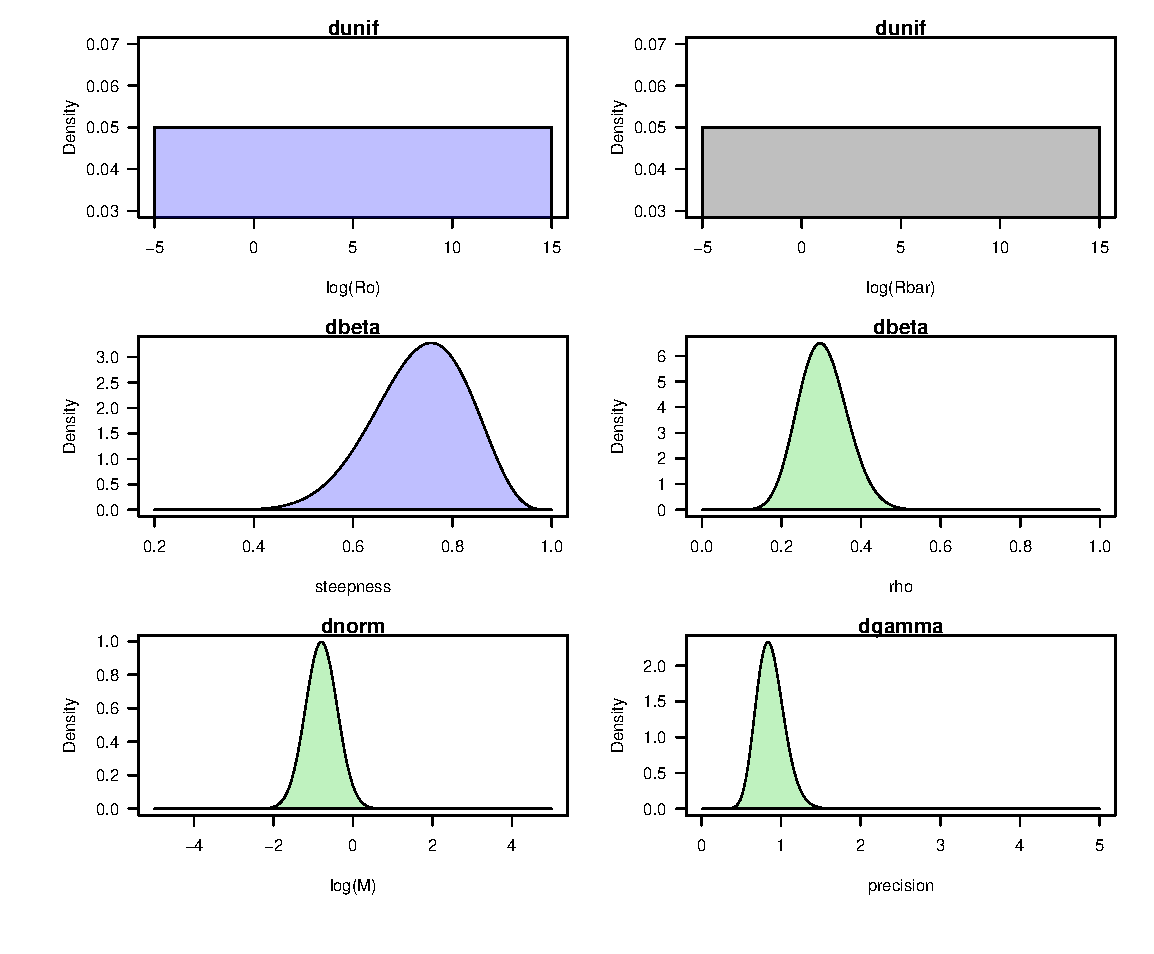
\includegraphics[width=0.7\textwidth]{../FIGS/qPriorFigs/iscam_fig_theta_prior_density.pdf}
		\caption{Prior densities for leading model parameters.}
		\label{fig:priors}
	\end{figure}
\end{frame}

% section analyticalmethods (end)




















